\documentclass[acmsmall,screen]{acmart}

\bibliographystyle{ACM-Reference-Format}
\citestyle{acmnumeric}

%% typeset pseudocode
\usepackage{algorithm}
\usepackage[noend]{algpseudocode}
\renewcommand{\algorithmicrequire}{\textbf{Input:}}
\renewcommand{\algorithmicensure}{\textbf{Output:}}

%% Some recommended packages.
\usepackage{booktabs}   %% For formal tables:
                        %% http://ctan.org/pkg/booktabs
\usepackage{subcaption} %% For complex figures with subfigures/subcaptions
                        %% http://ctan.org/pkg/subcaption

\usepackage[english]{babel}
\usepackage{bookmark}
\usepackage[utf8]{inputenc}
\usepackage[T1]{fontenc}
% \usepackage{lmodern}
\usepackage{xspace}
\usepackage{fancyhdr}
\usepackage{tcolorbox}

% Haskell code snippets and useful shortcuts
\usepackage{minted}
\setminted[haskell]{escapeinside=@@}
\newcommand{\hs}{\mintinline{haskell}}
\newcommand{\subhs}{\mintinline[fontsize=\small]{haskell}}
\newcommand{\cmd}[1]{\textsf{\color[rgb]{0,0,0.5} #1}}
\newcommand{\teq}{\smaller $\sim$}
\newcommand{\ghci}{$\lambda$>}
\newcommand{\defeq}{\stackrel{\text{def}}{=}}
\newcommand{\dollar}{{\color[rgb]{0.40,0.40,0.40} \$}}
\newcommand{\std}[1]{{\color[rgb]{0,0.3,0} #1}}
\newcommand{\blk}[1]{{\color[rgb]{0,0,0} #1}}
\newcommand{\blu}[1]{{\color[rgb]{0,0,1.0} #1}}

% Questions and tasks
\newcommand{\q}[2]{\textbf{\color{blue} Question #1:} #2}
\newcommand{\todo}[2]{[\textbf{\color{red} #1:} #2]}

% Abbreviations for projects
% \newcommand{\Dune}{\textsc{Dune}\xspace}
% \newcommand{\Haxl}{\textsc{Haxl}\xspace}

\begin{document}

%% Title information
\title[Formal Verification of Spacecraft Control Programs]{Formal Verification
of Spacecraft Control Programs (Experience Report)}

\author{Georgy Lukyanov}
\affiliation{
  \institution{Newcastle University}
  \country{United Kingdom}
}
\email{g.lukyanov2@ncl.ac.uk}
\author{Andrey Mokhov}
\affiliation{
  \institution{Newcastle University}
  \country{United Kingdom}
}
\email{andrey.mokhov@ncl.ac.uk}
\author{Jakob Lechner}
\affiliation{
  \institution{RUAG Space GmbH}
  \country{Austria}
}
\email{jakob.lechner@gmx.net}

% Don't forget \thispagestyle{firstpagestyle} after \maketitle
% \fancypagestyle{firstpagestyle}
% {
%    \fancyhf{}
%    \renewcommand{\headrulewidth}{0.2pt}
%    \fancyhead[C]{Under review, feedback is sought}
% }

\begin{abstract}
Verification of correctness of control programs is an essential task
in the development of space electronics; it is difficult and typically
outweighs design and programming tasks in terms of development hours.
This experience report presents a verification approach designed to help
spacecraft engineers reduce the effort required for formal verification of
low-level control programs executed on custom hardware.

% The approach uses a
% metalanguage to describe the semantics of a program as a state transformer,
% which can be compiled to multiple targets for testing, formal verification, and
% code generation. The metalanguage is embedded in Haskell, providing a way to
% prove some properties at the type level, which can shorten the feedback loop
% and further increase the productivity of engineers.

The verification approach is demonstrated on an industrial case study.
We present REDFIN, a processing core used in space missions, and its formal
semantics expressed using the proposed metalanguage for state transformers,
followed by examples of verification of simple control programs.

\keywords{formal verification, instruction set architecture, functional
programming, domain-specific languages.}
\end{abstract}

\keywords{}

\maketitle
% \thispagestyle{firstpagestyle}

\section{Introduction}\label{sec-intro}
Software bugs play a major role in the history of spacecraft
accidents~\cite{Leveson2004}. Some mission-ending bugs, e.g. those due to
software updates, would have been difficult to prevent, but plain integer
overflows~\cite{bug-rocket} and incorrect unit
conversion~\cite{NASA:1999:Mars} should have been eradicated long ago.
This paper
combines known formal verification and programming languages techniques and presents
a formal verification approach for simple control tasks, such as satellite power
management, which are executed on a real processing core used in space missions.

% Alas, there is no silver bullet. Testing is supported by mature methodologies
% and frameworks, but does not provide the full correctness guarantee. General-purpose
% strongly-typed languages can be used to eliminate important classes of bugs, but
% are less familiar to software engineers and are often not suitable for highly
% resource-constrained microarchitectures used in space electronics. Formal modelling
% methods provide a systematic approach for developing complex systems in a
% correct-by-construction manner, but they are still at the bleeding-edge of
% computing science and can be difficult to apply to real-life systems.

% We believe the presented ideas are transferable to other domains with similar
% safety and resource requirements, e.g. biomedical applications.

\begin{figure}
\centerline{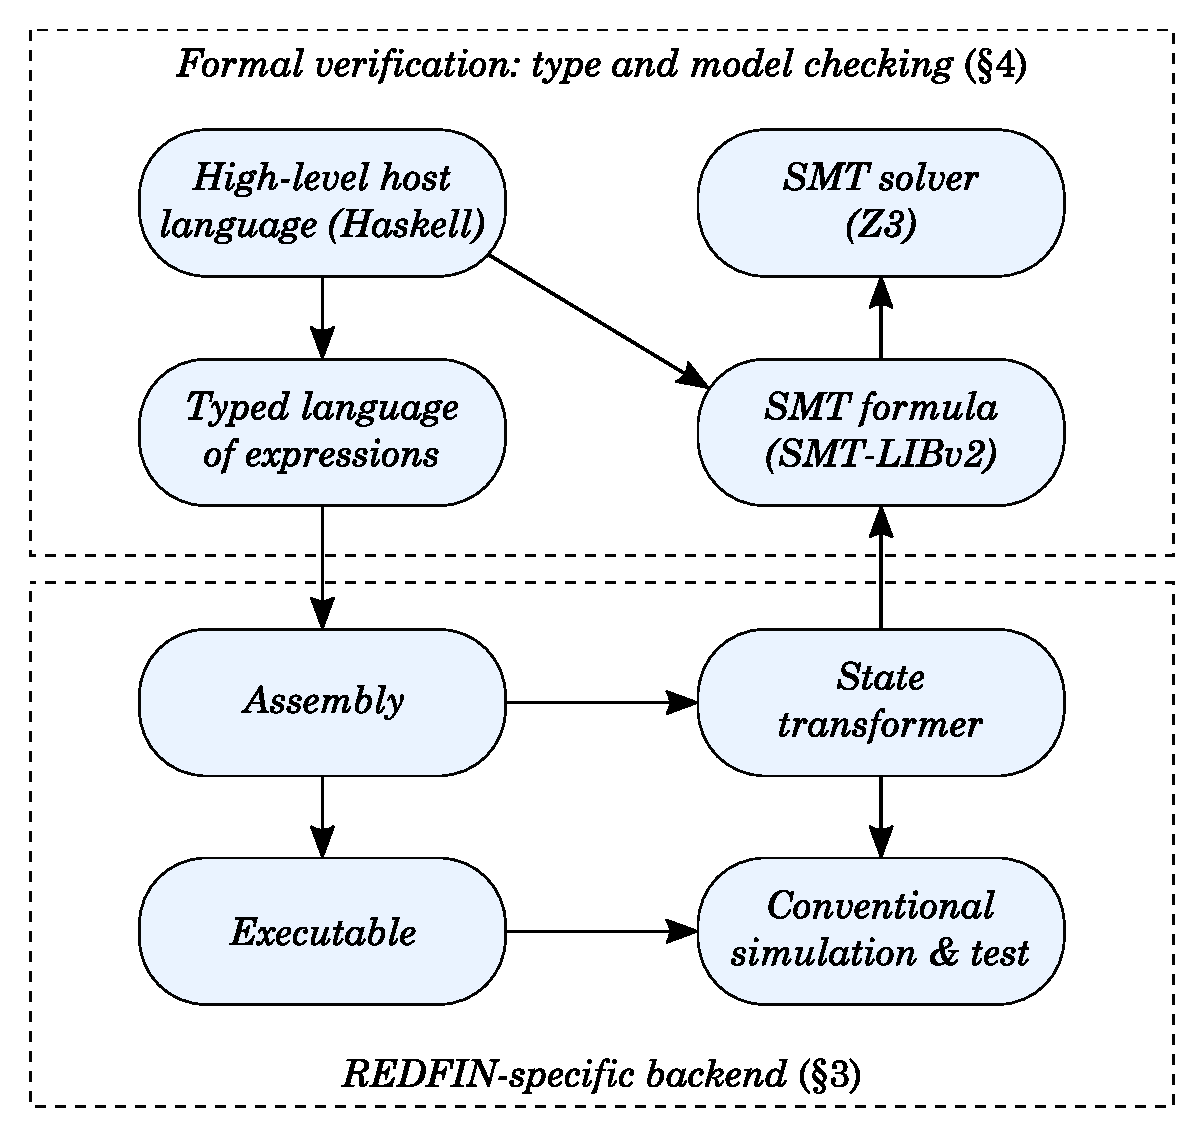
\includegraphics[scale=0.42]{fig/overview.pdf}}
\caption{Overview of the presented verification approach.\label{fig-overview}}
\end{figure}

Fig.~\ref{fig-overview} shows an overview of our approach. The bottom part
corresponds to conventional code generation and simulation, where
REDFIN\footnote{REDFIN stands for `REDuced instruction set for Fixed-point \&
INteger arithmetic'. This instruction set and the corresponding processing core
were developed by (Company Name) for space missions.
% RUAG Space Austria GmbH
See~\S\ref{sec-redfin} for more details.} assembly language is executed by
simulating the effect of each instruction on the state of the processor and memory.
The corresponding \emph{state transformer} is typically implicit and intertwined
with the rest of the simulation infrastructure. The main idea of our approach is
to represent the state transformer explicitly so that it can be symbolically
manipulated and used not only for simulation but also for formal verification.
The latter is achieved by compiling state transformers to SMT formulas and using
an SMT solver, e.g. Z3~\cite{de2008z3}, to verify that certain correctness
properties hold, for example, that integer overflow cannot occur regardless of
input parameters and that the program always terminates within stated time.

By using Haskell as the host language we can readily implement compilers from
higher-level \emph{typed} languages to untyped assembly, eradicating incorrect
number and unit conversion bugs. As shown at the top of Fig.~\ref{fig-overview},
engineers can write high-level control programs for the REDFIN architecture
directly in a small subset of Haskell. These high-level programs can be used for
type-safe code generation and as executable specifications of intended
functionality for the purposes of program synthesis and equivalence checking.

% To facilitate whole-program verification, we use a specific flavour of
% symbolic execution known as \emph{symbolic execution with merging}. In this approach,
% whenever a branch in the program is encountered, the symbolic execution engine performs
% merging of the two resulting disjunctive states, thus producing linear traces which could
% be translated into singular SMT-formulas representing whole programs. We refrain from a
% wider discussion of symbolic execution techniques here and refer the interested reader to
% the following survey paper~\cite{SurveySymExec-CSUR18}.

We first introduce the REDFIN processing core (\S\ref{sec-redfin}), then
present our verification approach (\S\ref{sec-transformer}-\S\ref{sec-verification}),
and conclude by a discussion (\S\ref{sec-discussion}) and a review of related
work (\S\ref{sec-related}).

% For many spacecraft subsystems integrated circuits are required to perform control
% tasks or simple data processing. Typically, these integrated circuits are realised
% with FPGAs (Field Programmable Gate Arrays) due to their flexibility and lower
% costs compared to ASIC (Application-Specific Integrated Circuit) development \&
% fabrication. Since FPGAs can be used to implement arbitrary circuit functions
% including processor cores, it is possible to perform tasks both in hardware and
% in software. However, modern space-qualified FPGAs, which can withstand radiation
% in Earth orbit or deep space, have a limited amount of programmable resources.
% Therefore, it is often not feasible to implement a fully-fledged processor system
% in such an FPGA next to the mission-specific circuitry.

Many spacecraft subsystems rely on integrated circuits to perform control tasks
or simple data processing. Typically, these integrated circuits are realised
with Field Programmable Gate Arrays (FPGAs) benefiting from their flexibility
and low cost. Modern space-qualified FPGAs that can withstand radiation in Earth
orbit or deep space have a limited amount of programmable resources, and it is
often not feasible to implement a fully-fledged processor system in such an FPGA
next to the mission-specific circuitry.
The REDFIN instruction set was developed to address this issue and meet the
following goals: (i)~simple instruction set with a small hardware footprint,
(ii)~reduced complexity to support formal verification of programs, and
(iii)~deterministic real-time behaviour.

\subsection{REDFIN instruction set and microarchitecture}
\vspace{-0.5mm}

REDFIN instructions have a fixed width of 16 bits.
The instruction set is based on a register-memory architecture, i.e.
instructions can fetch their operands from registers as well as directly from the
memory. This architecture favours a small register set, which minimises the hardware
footprint of the processing core. Furthermore, the number of instructions in a
program is typically smaller in comparison to traditional load/store architectures
where all operands have to be transferred to registers before any operations can
be performed. There are 47 instructions of the following types:

\vspace{-0.5mm}
\begin{itemize}
\item{Load/store instructions for moving data between registers and memory, and
loading of immediate values.}
\item{Integer and fixed-point arithmetic operations.}
% In the latter
% case the number of fractional bits can be adjusted by a processor register.
\item{Bitwise logical and shift operations.}
\item{Control flow instructions and comparison operations.}
\item{Bus access instructions for read \& write operations on an AMBA AHB bus
(not covered in this paper).}
\end{itemize}
\vspace{-0.5mm}

The REDFIN processing core fetches instruction and data words from a small and fast
on-chip SRAM. This only allows for execution of simple programs, however, it also
eliminates the need to implement caches and thus removes a source of non-determinism of
conventional processors. High performance is not one of the main goals, hence the
core is not pipelined and does not need to resolve data/control hazards or
perform any form of speculative execution. These properties greatly simplify
worst case execution time analysis.

\vspace{-1.2mm}
\subsection{Requirements for formal verification}
\vspace{-0.5mm}

Verification of \emph{functional correctness} of REDFIN programs, as defined by a
requirement specification, clearly is an essential task for the development of space
electronics. There are also important \emph{non-functional requirements}, such as
worst case execution time and energy consumption, which rely on the implementation
guarantees provided by the processing core. To reduce verification complexity,
the REDFIN core only allows to execute a single subroutine whose execution is triggered
by a higher-level controller in the system. The implementation guarantees that
concurrent bus accesses to the processor registers or memory do not affect
the subroutine execution time. Furthermore, the processor does not implement
interrupt handling. All these measures are taken to provide real-time
subroutine execution guarantees and make the verification of non-functional
properties feasible. % within the presented verification framework.

Despite these restrictions the REDFIN core has already proven its effectiveness for
simple control tasks and arithmetic computations as part of an antenna pointing unit
for satellites. Nevertheless, verification can be difficult and time-consuming,
even for small and simple programs. Verification activities, following engineering
standards for space electronics, typically outweigh programming and design tasks by a
factor of two in terms of development hours. Usually verification is performed via
program execution on an instruction set simulator or a hardware model of the processor.
Manually deriving test cases from the specification is cumbersome and error-prone
and simulation times can become prohibitively long with a large number of tests that
are often needed to reach the desired functional and code coverage. Formal verification
methods can prove that a program satisfies certain properties for all possible
test cases and are therefore immensely valuable for completing the verification
with superior efficiency and quality.

\section{Modelling REDFIN in Haskell\label{sec-transformer}}


In this section we formally define the REDFIN microarchitecture and express the
semantics of the instruction set as an explicit and symbolic state transformer.

\begin{figure}[t]
\begin{minted}[fontsize=\small]{haskell}
data State = State
  { registers           :: RegisterBank
  , memory              :: Memory
  , instructionCounter  :: InstructionAddress
  , instructionRegister :: InstructionCode
  , program             :: Program
  , flags               :: Flags
  , clock               :: Clock }
\end{minted}
\vspace{0.5mm}
\begin{minted}[fontsize=\small]{haskell}
type Register           = SymbolicValue Word2
type Value              = SymbolicValue Int64
type RegisterBank       = SymbolicArray Word2 Int64
type MemoryAddress      = SymbolicValue Word8
type Memory             = SymbolicArray Word8 Int64
\end{minted}
\vspace{0.5mm}
\begin{minted}[fontsize=\small]{haskell}
type InstructionAddress = SymbolicValue Word8
type InstructionCode    = SymbolicValue Word16
type Program            = SymbolicArray Word8 Word16
\end{minted}
\vspace{0.5mm}
\begin{minted}[fontsize=\small]{haskell}
data Flag               = Condition@\,@|@\,@Overflow@\,@|@\,@Halt@\,@...
type Flags              = SymbolicArray Flag Bool
type Clock              = SymbolicValue Word64
\end{minted}
\vspace{-2.5mm}
\caption{Basic types for modelling REDFIN.\label{fig-types}}
\vspace{-4.5mm}
\end{figure}

\subsection{The REDFIN Microarchitecture State}

The main idea of our approach is to use an explicit state transformer
semantics of the REDFIN microarchitecture. The \hs{State} of the entire
processing core is a product of states of every component, see
Fig.~\ref{fig-types}. We define \hs{SymbolicValue} and \hs{SymbolicArray} on top
of the SBV library~\cite{SBV} that we use as a frontend for SMT translation and
verification.

% \begin{equation*}
% \begin{split}
% S=\{(r, m, ic, ir, p, f, c) : r \in R, m \in M, ic \in A, \\ir \in I,
% p \in P, f \in F, c \in C\},
% \end{split}
% \end{equation*}

% \noindent
% where $R$ is the set of register bank configurations;
% $M$ is the memory state space;
% $A$~is the set of instruction addresses (the instruction counter $ic$ stores the
% address of the current instruction);
% $I$ is the set of instruction codes (the instruction register $ir$ stores the
% code of the current instruction);
% $P$ is the set of programs;
% $F$ is the set of the flag register configurations; and
% $C$ is the set of clock values.

% Fig.~\ref{fig-types} shows the translation of the above into Haskell types. Note
% that the types are not parameterised: recall that REDFIN is parameterised, e.g.
% the data width can be chosen depending on mission requirements, whereas we use fixed
% 64-bit data path for the sake of simplicity. The chosen names are self-explanatory,
% for example, the data type \hs{State} directly corresponds to the set of states~$S$.

% \todo{In principle, any other SMT frontend
% can be used, but to the best of our knowledge, SBV is the most mature SMT library
% available for Haskell. \textbf{No, SBV here is crucial because it does all the actual symbolic execution}} We briefly overview all \hs{State} components below.

% \subsubsection{Data values, registers and memory}

There are~4 registers (addressed by \hs{Word2}) and 256 memory cells (addressed
by \hs{Word8}) that store 64-bit values (\hs{Int64}). The register bank and
memory are represented by symbolic arrays
that can be accessed via SBV's functions \hs{readArray} and \hs{writeArray}.
REDFIN uses 16-bit \hs{InstructionCode}s, whose 6 leading bits contain the
opcode, and the remaining 10 bits hold instruction arguments. The \hs{Program}
maps 8-bit instruction addresses to instruction codes.

The microarchitecture status \hs{Flags} support conditional branching, track
integer overflow, and terminate the program (we omit a few other flags for
brevity).
The \hs{Clock} is a 64-bit counter
incremented on each clock cycle. Status flags and the clock are used for
diagnostics, formal verification, and worst-case execution time analysis.

\subsection{Instruction and Program Semantics}

We can now define the formal semantics of REDFIN instructions and programs as a
\emph{state transformer} $T : S \rightarrow S$, i.e. a function that maps
states to states. We distinguish instructions and programs by using
Haskell's list notation, e.g. $T_{\subhs{nop}}$ is the semantics of the
instruction $\hs{nop} \in I$, whereas $T_{\subhs{[}\subhs{nop}\subhs{]}}$ is the
semantics of the single-instruction program $\hs{[}\hs{nop}\hs{]} \in P$.

% \footnote{REDFIN does not have a dedicated \hs{nop}
% instruction, but one can use the semantically equivalent instruction \hs{jmpi 0}
% instead (i.e. jump to the next instruction).}

\vspace{-1.5mm}
\noindent\hrulefill~\\
\vspace{-3.5mm}

\noindent
\textbf{Definition (program semantics):} The semantics of a program $p \in P$
is inductively defined as follows:

% \begin{itemize}
% \item
    The semantics of the \emph{empty program} $\hs{[}\hs{]} \in P$ coincides with
    the semantics of the instruction \hs{nop} and is the identity state transformer:
    $T_{\subhs{[}\subhs{]}} = T_{\subhs{nop}} = \hs{id}$.

    % \item
    The semantics of a \emph{single-instruction program} $\hs{[}\hs{i}\hs{]} \in P$
    is a composition of (i) fetching the instruction from
    the program memory~$T_\textit{fetch}$, (ii) incrementing the
    instruction counter~$T_\textit{inc}$, and (iii) the state transformer
    of the instruction itself~$T_{\subhs{i}}$; or,~using the order of state
    components from Fig.~\ref{fig-types}:
    \vspace{-1mm}
    \[
    \begin{array}{lcl}
    T_\textit{fetch} & = & (r, m, ic, ir, p, f, c) \mapsto (r, m, ic, p[ic], p, f, c + 1)\\
    T_\textit{inc} & = & (r, m, ic, ir, p, f, c) \mapsto (r, m, ic + 1, ir, p, f, c)\\
    T_{\subhs{[}\subhs{i}\subhs{]}} & = & T_{\subhs{i}} \circ T_\textit{inc} \circ T_\textit{fetch}\\
    \end{array}
    \]

    % \item
    % \vspace{-1mm}
    \noindent
    The semantics of a \emph{composite program} $\hs{i}\hs{:}\hs{p} \in P$,
    where the operator~\hs{:}~prepends an instruction $\hs{i} \in I$ to a program
    $\hs{p} \in P$, is defined as $T_{\subhs{i}\subhs{:}\subhs{p}} = T_{\hs{p}} \circ T_{\subhs{[}\subhs{i}\subhs{]}}$.

% \end{itemize}

\vspace{-1mm}
\noindent\hrulefill~\\
\vspace{-3mm}

% \noindent
We represent state transformers in Haskell using the \emph{state monad}, a
classic approach to emulating mutable state in a purely functional programming
language~\cite{wadler1990comprehending}. We call our state monad~\hs{Redfin} and
define it as follows:
% \footnote{A generic version of this monad is available in standard module
% \hs{Control.Monad.State}.}

\vspace{0.5mm}
\begin{minted}[fontsize=\small]{haskell}
data Redfin a = Redfin
     { transform :: State -> (a, State) }
\end{minted}
\vspace{0.5mm}

\noindent
A computation of type~\hs{Redfin}~\hs{a} yields a value of type~\hs{a}~and
possibly alters the \hs{State} of the REDFIN microarchitecture.
The type \hs{Redfin}~\hs{()} describes a computation that does not produce any
value as part of the state transformation; such computations directly correspond
to state transformers.

\noindent
For example, here is the state transformer $T_\textit{inc}$:

\begin{minted}[fontsize=\small]{haskell}
incrementInstructionCounter :: Redfin ()
incrementInstructionCounter =
    Redfin $ \current -> ((), next)
  where
    next = current { instructionCounter =
        instructionCounter current + 1 }
\end{minted}

\noindent
In words, the state transformer looks up the value of the \hs{instructionCounter}
in the \hs{current} state and replaces it in the \hs{next} state with the
incremented value. We can compose such primitive computations into more complex
state transformers using Haskell's \hs{do}-notation:

\begin{minted}[fontsize=\small]{haskell}
readInstructionRegister :: Redfin InstructionCode
readInstructionRegister =
    Redfin $ \s -> (instructionRegister s, s)
\end{minted}

\begin{minted}[fontsize=\small]{haskell}
executeInstruction :: Redfin ()
executeInstruction = do
    fetchInstruction
    incrementInstructionCounter
    instructionCode <- readInstructionRegister
    decodeAndExecute instructionCode
\end{minted}

\noindent
Here \hs{readInstructionRegister} reads the instruction code from the current
state \emph{without modifying it}, and is subsequently used in \hs{executeInstruction},
which defines the semantics of the REDFIN execution cycle. We omit definitions of
\hs{fetchInstruction} and \hs{decodeAndExecute} for brevity. The latter is a
case analysis of 47 opcodes that returns the matching instruction. We discuss
several instructions below.

\subsubsection{Halting the Processor}
The instruction~\hs{halt} sets the flag~\hs{Halt}, thereby stopping the
execution of the current subroutine until a new one is started by a higher-level
system controller that resets \hs{Halt}.

\begin{minted}[fontsize=\small]{haskell}
halt :: Redfin ()
halt = writeFlag Halt true
\end{minted}

\noindent
The auxiliary function \hs{writeFlag} modifies the flag:

\begin{minted}[fontsize=\small]{haskell}
writeFlag :: Flag -> SymbolicValue Bool -> Redfin ()
writeFlag flag value = Redfin $ \s -> ((), s')
  where
    s' = s { flags =
        writeArray (flags s) (flagId flag) value }
\end{minted}

\noindent
In the rest of the paper we will use auxiliary functions \hs{readRegister},
\hs{writeRegister}, \hs{readState}, etc.; they are simple state transformers
defined similarly to \hs{writeFlag}.

\subsubsection{Arithmetics}
The instruction \hs{abs} is more involved:
it reads a register and writes back the absolute value of its contents.
The semantics accounts for the potential integer overflow that leads to the
\emph{negative resulting value} when the input is $-2^{63}$ (REDFIN uses the
common two's complement signed number representation). The overflow is flagged
by setting~\hs{Overflow}. We use SBV's symbolic \emph{if-then-else}
operation~\hs{ite} to \emph{merge} two symbolic values~---~in this case two
possible next states, one of which is a state with the \hs{Overflow} flag set:

\begin{minted}[fontsize=\small]{haskell}
abs :: Register -> Redfin ()
abs reg = do
    state  <- readState
    result <- fmap Prelude.abs (readRegister reg)
    let (_, state') =
      transform (writeFlag Overflow true) state
    writeState $ ite (result .< 0) state' state
    writeRegister reg result
\end{minted}

\subsubsection{Conditional Branching}
As an example of a control flow instruction consider \hs{jmpi_ct}, which
tests the~\hs{Condition} flag, and adds the provided \hs{offset} to the
instruction counter if the flag is set.

\begin{minted}[fontsize=\small]{haskell}
jmpi_ct :: SymbolicValue Int8 -> Redfin ()
jmpi_ct offset = do
    ic <- readInstructionCounter
    condition <- readFlag Condition
    let ic' = ite condition (ic + offset) ic
    writeInstructionCounter ic'
\end{minted}

\noindent
% After working through the above examples, it is worth noting that
We use our Haskell encoding of the state transformer as a~\emph{metalanguage}:
we operate the REDFIN core as a puppet master, using external meta-notions of
addition, comparison and let-binding. From the processor's
point of view, we have infinite memory and act instantly, which gives us unlimited
modelling power. For example, we can simulate the processor environment
in an external tool and feed its result to \hs{writeRegister} as if it was
obtained in one clock cycle.

\subsection{Symbolic simulation}

Having defined the semantics of REDFIN programs, we can perform
\emph{symbolic processor simulation}.

There are many flavours of symbolic execution~\cite{SurveySymExec-CSUR18}
and there is no single answer to the question of which one is the best.
The choice of the symbolic execution technique depends heavily on the
verification scenarios. The verification framework for REDFIN is designed
to deal with two main classes of programs: (i) arithmetic calculations that
are statically provable to be terminating and (ii) control programs with
unbounded loops whose termination depend on dynamic input data. We approach
verification of the former using~\emph{symbolic execution with merging} that
allows for whole-program verification by translating the program and the
verification condition into a single SMT formula. However, unconditional merging
does not work for non-terminating programs; thus
we employ the traditional approach to symbolic execution that generates from programs
the tree-shaped traces which could be split into separate execution paths for path-by-path
analysis and verification. The verification framework thus works in two
modes:~\emph{merging} and~\emph{branching}. See section~\ref{sec-verification} for
a verification example using the merging mode and section~\ref{sec-motor-control} for
an approach to verify a non-terminating program in branching mode.

\subsubsection{Merging Mode}

The function \hs{simulate} takes a number of simulation
steps~$N$ and an initial symbolic \hs{State} as input, and executes
\hs{executeInstruction} defined above $N$ times. In each \hs{state} we
merge two possible futures: (i) if the \hs{Halt} flag is set, we continue the
simulation from the \hs{next} state, (ii) otherwise we remain in the current
\hs{state}, since in this case the processor must remain idle.

\begin{minted}[fontsize=\small]{haskell}
simulate :: Int -> State -> State
simulate steps s
  if steps <= 0
  then s
  else ite halted s (simulate (steps - 1) next)
 where halted = readArray (flags s) (flagId Halt)
       next   = snd (transform executeInstruction s)
\end{minted}

The function~\hs{ite} here performs symbolic merging of two possible states:
where the halted flag is set and not. The underlying semantics of instructions
will also perform merging on encounter of every branching instruction.

\subsubsection{Branching Mode}

In branching mode, on the contrary, we do not perform any merging at all and generate a
rose tree\footnote{As defined in~\hs{Data.Tree} module of Haskell's~\texttt{containers} package}-shaped
symbolic execution trace where every node stores an integer identifier, a program state and its
associated path constraints.
We take advantage of the fact that the semantics of the~\hs{halt}
instruction updates the~\hs{Halt} flag with concrete boolean value~\hs{True} and thus we
can use the native Haskell conditional operator to check if the current execution path
has terminated and return a leaf node in this case. Otherwise, we generate~\hs{children} --- a list of
successor states, recursively calling the~\hs{simulate} function with every child as the initial state
and attaching the results as leaves to the current node.

\begin{minted}[fontsize=\small]{haskell}
simulate :: Int -> State -> Tree (Node Int State)
simulate steps s = getTrace $ do
    modify (+ 1)
    n <- get
    let halted = readArray (flags s) (flagId Halt)
    if steps <= 0 || halted
    then pure (mkTrace (Node n s) [])
    else do children <- traverse (simulate (steps - 1)) (executeInstruction s)
            pure $ mkTrace (Node n s) children
\end{minted}

Symbolic simulation is very powerful. It allows us to formally verify properties
of REDFIN programs by fixing some parts of the state to constant values (e.g.,
the program), and then making assertions on the resulting values of
the symbolic part of the state, as demonstrated in the next
sections~\S\ref{sec-verification} and~\S\ref{sec-motor-control}.

\section{Formal verification\label{sec-verification}}
This section presents the formal verification framework developed on top of
the REDFIN semantic core (\S\ref{sec-transformer}) demonstrating the following
steps of the workflow:

\begin{itemize}
    \item Develop programs in low-level REDFIN assembly, and in a high-level
    typed language embedded in Haskell.
    \item Test REDFIN programs on concrete input values.
    \item Define functional correctness and worst case execution time properties
    in the SBV property language.
    \item Verify the properties or obtain counterexamples.
\end{itemize}

\noindent
Consider the following simple spacecraft control task.

\begin{tcolorbox}
Let $t_1$ and $t_2$ be two different time points (measured in ms),
and $p_1$ and $p_2$ be two power values (measured in mW).
Calculate the estimate of the total energy consumption during this period
using linear approximation, rounding down to the nearest integer:
\[
\textit{energyEstimate}(t_1, t_2, p_1, p_2) = \left\lfloor \frac{|t_1 - t_2| * (p_1 + p_2)}{2} \right\rfloor.
\]
\end{tcolorbox}

\noindent
This task looks too simple, but in fact it has a few pitfalls that,
if left unattended, may lead to the failure of the space mission. Examples
of subtle bugs in seemingly simple programs leading to a catastrophe include 64-bit
to 16-bit number conversion overflow causing the destruction of Ariane~5
rocket~\cite{bug-rocket} and the loss of NASA's Mars orbiter due to incorrect
unit conversion~\cite{NASA:1999:Mars}. Let us develop and verify
a REDFIN program for this task.

% \subsubsection{Writing the program}
We can write programs in the untyped REDFIN assembly, or in a typed higher-level
expression language. The former allows engineers to hand-craft highly optimised
programs under tight resource constraints, while the latter brings type-safety
and faster prototyping. We start with the high-level approach and define an
expression that can be used both as a Haskell function and a high-level REDFIN
expression:

% Using Haskell's polymorphism, we can

\begin{minted}[fontsize=\small]{haskell}
energyEstimate :: Integral a => a -> a -> a -> a -> a
energyEstimate t1 t2 p1 p2 =
    abs (t1 - t2) * (p1 + p2) `div` 2
\end{minted}

\noindent
Thanks to polymorphism, we can treat \hs{energyEstimate} both as a numeric
function, and as an abstract syntax tree that can be \emph{compiled} into a
REDFIN assembly \hs{Script}. Due to the lack of space we omit the implementation
of \hs{Script}, but one can think of it as a restricted version
of the \hs{Redfin} state transformer, which we use to write \emph{programs that
can manipulate the processor state only by executing instructions}, e.g. the
only way to set the \hs{Overflow} flag is to execute an arithmetic instruction
that might cause an overflow.

\begin{minted}[xleftmargin=10pt,fontsize=\small]{haskell}
energyEstimateHighLevel :: Script
energyEstimateHighLevel = do
  let t1    = read (IntegerVariable 0)
      t2    = read (IntegerVariable 1)
      p1    = read (IntegerVariable 2)
      p2    = read (IntegerVariable 3)
      temp  = Temporary 4
      stack = Stack 5
  compile r0 stack temp (energyEstimate t1 t2 p1 p2)
  halt
\end{minted}
\label{energyEstimateHighLevel}

\noindent
Here the type \hs{IntegerVariable} is used to statically distinguish between integer
and fixed-point numbers, \hs{Temporary} to mark temporary words, so they cannot
be mixed with inputs and outputs, and \hs{Stack} to denote the location of the
stack pointer. The~\hs{let} block declares six adjacent memory addresses: four
input values $\{t_1, t_2, p_1, p_2\}$, a temporary word and a stack pointer.
We~\hs{compile} the high-level expression \hs{energyEstimate} into the assembly
language by translating it to a sequence of REDFIN instructions. The first
argument of the~\hs{compile} function holds the register~\hs{r0} which contains
the estimated energy value after the program execution.

% \subsubsection{Simulating the program}
We can run symbolic simulation for 100 steps, initialising the program and data
memory of the processor using the function \hs{simulate} defined above and a
helper function \hs{boot}.

\begin{minted}[xleftmargin=10pt,fontsize=\small]{haskell}
main = do
  let dataMemory = [10, 5, 3, 5, 0, 100]
      finalState = simulate 100 $
        boot energyEstimateHighLevel dataMemory
  printMemoryDump 0 5 (memory finalState)
  putStrLn $ "R0: " ++ show
             (readArray (registers finalState) r0)
\end{minted}

\noindent
As the simulation result we get a \hs{finalState}. We inspect it by
printing relevant components: the values of the first six memory cells, and the
result of the computation located in the register~\hs{r0}. Note that the stack
pointer (cell 5) holds 100, as in the initial state, which means the stack is empty.

\begin{minted}[frame=single, fontsize=\small]{text}
Memory dump: [10, 5, 3, 5, 5, 100]
R0: 20
\end{minted}

Simulating programs with specific inputs is useful for diagnostic and test, but
SMT solvers allow us to verify the correctness for \emph{all valid input
combinations}. To demonstrate this, let us discover a problem in our energy
estimation program. Consider the following correctness property.

% \subsubsection{Verifying the program}
% The project lead engineer defined a set of functional requirements for the
% energy monitoring subsystem. The software engineering team received the
% specification, implemented the energy monitoring subroutines, and started the
% verification. One of the requirements is as follows.

\begin{tcolorbox}
Assuming that values $p_1$ and $p_2$ are non"/negative integers, the energy
estimation subroutine must always return a non-negative integer value.
\end{tcolorbox}

To check that the program meets this requirement, we translate
\hs{energyEstimateHighLevel} into an SMT formula,
and formulate the corresponding theorem:

\begin{minted}[fontsize=\small]{haskell}
theorem = do
  t1 <- forall "t1" -- Initialise symbolic variables
  t2 <- forall "t2"
  p1 <- forall "p1"
  p2 <- forall "p2" -- And then add constraints:
  constrain $ p1 .>= 0 &&& p2 .>= 0
  -- Initialise the data memory with symbolic variables:
  let dataMemory = [t1, t2, p1, p2, 0, 100]
      finalState = simulate 100
        (boot energyEstimateHighLevel dataMemory)
      result = readArray (registers finalState) r0
      halted = readArray (flags finalState) (flagId Halt)
  return $ halted &&& result .>= 0
       &&& result .== energyEstimate t1 t2 p1 p2
\end{minted}

\noindent
We extract the computed result and the value of the flag \hs{Halt} from the
\hs{finalState}, and then assert that the processor has halted, the result is
non-negative, and is equal to that computed by the high-level Haskell expression
\hs{energyEstimate}.
The resulting SMT formula can be checked by Z3 in
3.0s\footnote{We use a laptop with 2.90GHz Intel Core i5-4300U processor, 8GB
RAM (3MB cache), and the SMT solver Z3 version 4.5.1 (64-bit).}:

\begin{minted}[frame=single,fontsize=\small]{text}
> proveWith z3 theorem
Falsifiable. Counter-example:
  t1 = 5190405167614263295 :: Int64
  t2 =                   0 :: Int64
  p1 =  149927859193384455 :: Int64
  p2 =  157447350457463356 :: Int64
\end{minted}

%TODO: Can we obtain a simpler counterexample using SBV optimisation?
\noindent
Z3 has found a counterexample demonstrating that the program does not
satisfy the above property. Indeed, the expression evaluates to a negative
value on the provided inputs due to an \emph{integer overflow}. We therefore
refine the property:

\begin{tcolorbox}
According to the spacecraft power system specification, $p_1$ and $p_2$ are
non"/negative integers not exceeding 1W. The time is measured
from the mission start, hence $t_1$ and $t_2$ are non-negative and do not exceed
the time span of the mission, which is 30 years. Under these assumptions,
the energy estimation subroutine must return a non-negative integer value.
\end{tcolorbox}

\noindent
We need to modify time and power constraints accordingly:
% \footnote{We are not absolutely
% precise here. We do not distinguish between regular and leap years, and use
% a conservative upper bound of 366 days per year.}

\begin{minted}[xleftmargin=10pt,fontsize=\small]{haskell}
constrain $ p1 .<= toMilliWatts   ( 1 :: Watt)
        &&& t1 .<= toMilliSeconds (30 :: Year)
        &&& t1 .>= 0 &&& t2 .>= 0 &&& ... -- etc.
\end{minted}

\noindent
Rerunning Z3 produces the desired \textsf{QED} outcome in 4.8s.

The refinement has rendered the integer overflow impossible;
in particular, \hs{abs} can never be called with~$-2^{63}$
within the mission parameters. Such guarantee fundamentally requires
solving an SMT problem, even if it is done at the type level, e.g. using
\emph{refinement types}~\cite{vazou2014refinement}.

% \subsubsection{Checking program equivalence}
The statically typed high-level expression language is very convenient for
writing REDFIN programs, however, an experienced engineer can often find a way
to improve the resulting code. In some particularly resource-constrained situations,
a fully hand-crafted assembly code may be required. As an example, a direct
unoptimised translation of the \hs{energyEstimate} expression into assembly uses
79 instructions, most of them for \hs{Stack} manipulation.
On the other hand, it is not difficult to write a low-level assembly program that
computes the result using only 9 instructions:

\begin{minted}[xleftmargin=10pt,fontsize=\small]{haskell}
energyEstimateLowLevel :: Script
energyEstimateLowLevel = do
    let { t1 = 0; t2 = 1; p1 = 2; p2 = 3 }
    ld r0 t1
    sub r0 t2
    abs r0
    ld r1 p1
    add r1 p2
    st r1 p2
    mul r0 p2
    sra_i r0 1
    halt
\end{minted}
\label{energyEstimateLowLevel}

\noindent
To support the development of hand-crafted code, we use Z3 to \emph{check the
equivalence of REDFIN programs} by verifying that they produce
the same output on all valid inputs. This allows an engineer to
optimise a high-level prototype and have a guarantee that no bugs were
introduced in the process. The corresponding \hs{equivalence} check takes 11.5s.
% (on 52 SMT clauses)

% \begin{minted}[frame=single,fontsize=\small]{text}
% > proveWith z3 equivalence
% Q.E.D.
% \end{minted}

% Below we check the \hs{equivalence} of this low-level program with
% \hs{energyEstimateHighLevel} introduced earlier.

% \begin{minted}[xleftmargin=10pt,fontsize=\small]{haskell}
% equivalence = do
%   t1 <- forall "t1"
%   t2 <- forall "t2"
%   p1 <- forall "p1"
%   p2 <- forall "p2"
%   constrain $ p1 .>= 0 &&& p2 .>= 0
%       &&& p1 .<= toMilliWatts   ( 1 :: Watt)
%       &&& p2 .<= toMilliWatts   ( 1 :: Watt)
%       &&& t1 .>= 0 &&& t2 .>= 0
%       &&& t1 .<= toMilliSeconds (30 :: Year)
%       &&& t2 .<= toMilliSeconds (30 :: Year)
%   let memory   = [t1, t2, p1, p2, 0, 100]
%       llState  = simulate 100 (boot energyEstimateLowLevel  memory)
%       hlState  = simulate 100 (boot energyEstimateHighLevel memory)
%       llResult = readArray (registers llState) r0
%       hlResult = readArray (registers hlState) r0
%   return $ llResult .== hlResult
% \end{minted}

% \subsubsection{Program timing analysis}

Every call of the~\hs{executeInstruction} function advances the \hs{clock} field
of the \hs{State} (see Fig.~\ref{fig-types}) by the appropriate number of
cycles, precisely matching the hardware implementation. This allows us to
perform~\emph{best/worst case execution timing analysis} using the
optimisation facilities of SBV and Z3. As an example,
let us determine the minimum and maximum number of clock cycles required for
executing~\hs{energyEstimateLowLevel}. To make this example more
interesting, we modified the semantics of the instruction~\hs{abs} and
added~1~extra clock cycle in case of a negative argument.
% by conditionally performing
% \hs{delay 1} in the state transformer \hs{abs}.

% \begin{minted}{haskell}
% delay :: Clock -> Redfin ()
% delay cycles =
%     Redfin $ \s -> ((), s { clock = clock s + cycles })
% \end{minted}
%TODO: Same can be done about power

\begin{minted}[xleftmargin=10pt,fontsize=\small]{haskell}
timingAnalysis = optimize Independent $ do
  ... -- Initialise and run symbolic simulation
  minimize "Best case"  (clock finalState)
  maximize "Worst case" (clock finalState)
\end{minted}

\noindent
The total delay of the program depends only on the sign of $t_1 - t_2$, thus
the best and worst cases differ only by one clock cycle. The worst case is
achieved when the difference is negative ($t_1 - t_2 = -2$), as shown below.
Z3 finishes in 0.5s.

\noindent
\begin{minipage}{0.53\linewidth}
\begin{minted}[frame=single,fontsize=\small]{text}
Objective "Best case":
Optimal model:
  t1        = 549755813888
  t2        =  17179869184
  p1        =            0
  p2        =            0
  Best case =           12
\end{minted}
\end{minipage}
\begin{minipage}{0.46\linewidth}
\begin{minted}[frame=single,fontsize=\small]{text}
Objective "Worst case":
Optimal model:
  t1         = 65535
  t2         = 65537
  p1         =     0
  p2         =     0
  Worst case =    13
\end{minted}
\end{minipage}

\section{Formal verification in presence of unbounded loops\label{sec-motor-control}}

In the last section we have demonstrated the framework's capabilities for
formal verification on an example of the energy estimation program.
Many programs targeting REDFIN share the distinctive feature of
this example and have statically predictable upper \emph{bound on execution time}
thanks to the fact that their termination does not
depend on the input data. However, some control programs may have loops
which are guarded by termination conditions that involve computation
considering the input parameters of the program, thus making the loop
\emph{unbounded}.

The presence of unbounded loops makes whole-program
verification inapplicable in the general case~\cite{some-paper-on-symexec},
since the state space of the program becomes huge or even infinite. However,
if the program essentially comprises a single unbounded loop, some properties
of the program could be verified by determining the \emph{loop invariant}
and proving that it holds for every iteration of the loop.

In this section we apply the developed verification framework to a larger
example of a stepper motor control program and make an accent on how
the presence of an unbounded loop may be mitigated and which properties
of the program can be verified with symbolic execution.

\subsection{Stepper motor control program}

Stepper motors are often deployed as parts of antenna and solar panel pointing units
in space satellites. We consider a control program for controlling a motor with
one degree of freedom. The program, given the distance to move the motor and safety
bounds on velocity and acceleration, will compute a series of speed and velocity values
that can be used to move the motor.

The algorithm~\ref{alg-motor} expects three input
parameters: $dist$ --- the distance to move the motor, $v\_max$ --- the maximal permitted
velocity and $a\_max$ --- the maximal permitted acceleration. The conditional statement on
line 9 decided whether to accelerate the motor, to keep it on steady speed or to decelerate
it; see~\ref{fig-motor} for plots of velocity and distance travelled against time. The
spike on the bottom-left of the velocity graph illustrates the edge case when the $dist$
parameter is not divisible by $a\_max$ (\todo{check this bit}).

\begin{algorithm}[h]
  \label{alg-motor}
  \begin{algorithmic}[1]
\Require {$dist$, $v\_max$, $a\_max$}
\State $s \gets 0$
\State $v \gets 0$
\While {$true$}
  % Compute deceleration distance based on current speed
  \State $decel\_steps\gets \lfloor v / a\_max \rfloor$
  \algorithmiccomment{# Compute deceleration distance based on current speed}
  \State $s\_decel \gets a\_max \cdot (decel\_steps + 1) / 2$
  \If {$decel\_steps \cdot a\_max \neq v$}
    \State $s\_decel \gets s\_decel + v$
  \EndIf
  \State {$v\_next = min(v\_max, dist, v + a\_max)$}
  \If {$s + s\_decel + v\_next \leq dist$}
    \State $v \gets v\_next$ \algorithmiccomment{accelerate}
  \ElsIf {$s + s\_decel + v \leq dist$}
    \State $ v \gets v $     \algorithmiccomment{keep speed}
  \Else
     \algorithmiccomment{decelerate}
    \If {$v > decel\_steps \cdot a\_max$}
      \State $v \gets decel\_steps \cdot a\_max$
    \Else
      \State $v \gets v - a\_max$
    \EndIf
  \If {$v = 0$}
    \If {$s \neq dist$}  \algorithmiccomment{accelerate again to reach target}
      % didn't quite reach our target after deceleration
      % => accelerate again
      \State $v \gets min(dist - s, a\_max)$
    \Else
      % reached target
      \State $break$  \algorithmiccomment{terminate execution}
  \EndIf
\EndWhile
\end{algorithmic}
\caption{Motor Control Algorithm}
\end{algorithm}

\begin{figure}[h]
\centerline{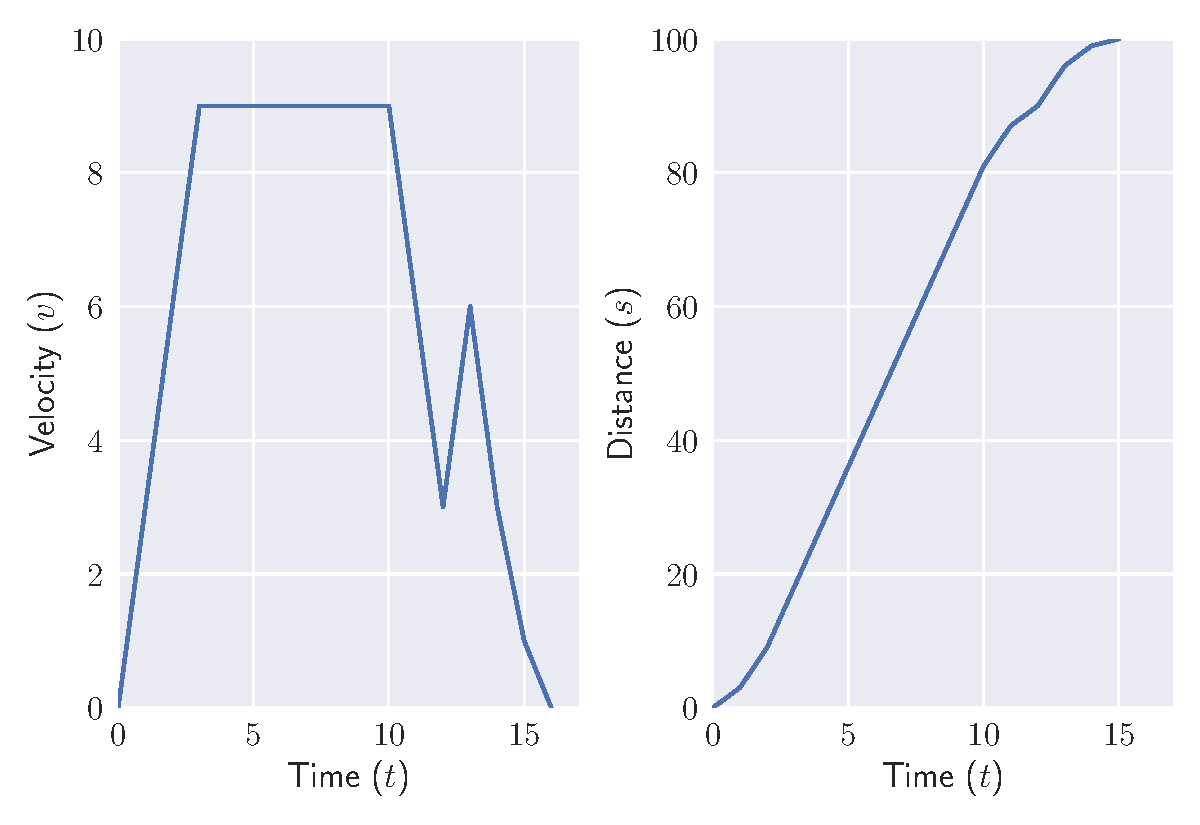
\includegraphics[scale=0.6]{fig/motor_control_graph.pdf}}
\caption{Motor control program execution\label{fig-motor}}
\Description[Please consult the text of this section for the description]{}
\end{figure}

To be deployed into Redfin, the algorithm~\ref{alg-motor} must be manually
re-implemented in Redfin assembly. The resulting assembly program comprises 85 lines of
code and mostly mirrors the pseudocode of the algorithm.

\subsection{Loop invariant verification}

In order to ensure that the motor will not introduce disturbances
and will not lead the whole unit out of its normal mode of operation, the velocity and
acceleration of the motor must be kept in safe limits. More formally, that would mean
that in any iteration of the loop the values of the expressions $v$, the velocity,
and $\left| v\_next - v \right|$, the acceleration, never exceed the
parameters $v\_max$ and $a\_max$,
respectively. This property is the loop invariant for the motor control program which
ensures that velocity and acceleration always stay within their safe bounds. We can
formalise it as the following predicate that quantifies over the program's inputs and
state:

\begin{figure}[h]
\[
  \forall\ v\_max\ a\_max\ v\ v\_next\ s,
  \ v\ \leq v\_max\ \land\ \left| v\_next - v \right| \leq a\_max
\]
\caption{Loop invariant: velocity and acceleration are within bounds}
\end{figure}

We will verify the loop invariant by using the verification framework in the
\emph{branching mode}\ref{sec-operation-modes}. While symbolic execution with
merging, which is implemented by the framework's \emph{mergin} mode, allows
for intuitive formulation of properties for whole-program verification and
is very useful for finite programs and programs with bounded loops, as we have
reported in the previous sections, in presence of branches that depended on
symbolic values it suppers from \emph{symbolic termination}. Thus, for verifying the
loop invariant, we rely on traditional symbolic execution.

To verify the loop invariant we take the following approach:

\begin{itemize}
  \item Obtain the binary tree-shaped trace by \emph{bounded} symbolic execution
  in \emph{branching} mode
  \item Split the trace into linear paths, thus enumerating all the possible
    execution scenarios
  \item For every path perform the analysis
    \begin{enumerate}
      \item Extract the relevant parts of the state from the \emph{last} node in
            the path, i.e. symbolic expressions stored in
            registers, memory cells or flags
      \item Construct a symbolic expression representing the \emph{property to check},
            which would involve the expressions obtained in the previous step
      \item Extract the \emph{path condition} from the /last/ node in the path
      \item Formulate the \emph{preconditions} of the program
      \item To verify the property in the given path by checking the following
            formula for satisfiability:
              preconditions /\ path constraints /\ ¬ property to check
    \end{enumerate}
    \item  The property holds if and only if for every path the solver returns
           \hs{Unsatisfiable}, i.e. there are no assignments of the variables which
           satisfy the~\emph{negation} of the property to check, considering the
           preconditions and the path condition.
\end{itemize}

This detailed verification algorithms has several parameters that need to be specified:

\begin{itemize}
\item Preconditions on $v\_max$ and $a\_max$
\item Symbolic execution bound, i.e. for how many steps perform the execution. Since the
      body of the loop will always terminate this bound can be calculated in advance.
\end{itemize}

Give the preconditions, an example of the execution path, talk about constant folding
and SMT-solving to prove unsatisfiable paths, make a table(?) with results for different
preconditions: number of path, time to solve a path, length of the path maybe.

\subsection{NOTES}

``Pre-conditions, when
available, may be leveraged to reduce the size of the input
data domains and to only generate test inputs that satisfy
the pre-conditions.''


---

\section{Discussion\label{sec-discussion}}
% The presented approach has been implemented and is planned to be released at the
% conference (this paper is currently under review).

% In this section we discuss our design choices and achieved
% results, comparing them with the project's initial goals: (i)~providing a unified
% specification, testing, and formal verification framework that is (ii)~understandable
% and convenient to use by the REDFIN engineering team, and (iii)~allows the team
% to co-develop REDFIN software and hardware, by extending and modifying the
% default instruction semantics.

% \subsection{From hardware to untyped assembly to typed software}

% The proposed approach covers two levels of organisation of computer systems: the
% hardware microarchitecture (the state monad \hs{Redfin},~\S\ref{sec-transformer}),
% and the instruction set architecture (the assembly monad
% \hs{Script},~\S\ref{sec-verification}). These two levels are very different: the
% former allows hardware engineers to precisely capture the semantics of
% instructions (and has proven useful in exposing underspecified behaviours),
% whereas the latter does not have a direct access to the microarchitectural level
% and is used to symbolically \emph{execute} the semantics, allowing software
% engineers to \emph{observe} the results and \emph{reason} about program
% correctness.

As the previous section~\S\ref{sec-verification} demonstrates, the presented
approach provides a unified specification, testing, and formal verification
framework. It allows the REDFIN engineering team to co-develop REDFIN software
and hardware, by extending and modifying the default instruction semantics.
By using Haskell as a metalanguage, one can implement higher-level languages on
top of the REDFIN assembly, such as our simple statically-typed language for
arithmetic expressions.

Static typing, polymorphism, \textsf{do}-notation, and availability of a mature
symbolic manipulation library~(SBV) were the key factors for choosing Haskell
for this project. We also have a prototype implementation in the
dependently-typed language Idris~\cite{JFP:9060502} that allows us to verify
more sophisticated properties at the type level, however at the time of writing
there is no equivalent of the SBV library in Idris, which is a significant
practical disadvantage.
% Dependent Haskell~\cite{weirich2017dependent} is a
% pos alternative.

% \subsection{Uniform development, testing and verification environment}

The \hs{Script} monad was engineered to provide familiar assembly mnemonics and
directives (e.g. labels), which allows engineers to start
using the framework for developing REDFIN programs even without prior Haskell
experience, hopefully increasing the uptake of the framework.

Thanks to symbolic simulation, we can uniformly handle both concrete and
symbolic values, reusing the same code base and infrastructure for testing and
formal verification.
Testing yields trivial SMT problems that can be solved in sub-second time.
Formal verification is more expensive: in our experiments,
programs of realistic sizes (typical REDFIN programs have hundreds of
instructions) required 10-15 minutes, but one can
easily construct tiny programs that will grind any SMT solver to a halt:
for example, analysis of a single multiplication instruction can take half an
hour if it is required to factor 64-bit numbers --- try to factor
4611686585363088391 with an SMT solver! In such cases, conservatively proving
some of the correctness properties at the type level can significantly increase
the productivity. As a microbenchmark, we verified the correctness of an array
summation program, reporting the number of SMT clauses and Z3 runtime for
low-level (LL) and high-level (HL) programs:

{\centering
\begin{tabular}{l||c|c|c|c|c}
\hline
Benchmark        & Array & Clauses & Clauses & Time    & Time    \\
                 & size  & LL      & HL      & LL      & HL      \\\hline
Overflow:        & 9     & 286     & 260     & 1.482s  & 0.443s  \\
values not       & 12    & 492     & 453     & 3.604s  & 1.365s  \\
constrained      & 15    & 740     & 688     & 49.969s & 7.362s  \\
                 & 18    & 1030    & 965     & 76.757s & 88.458s \\\hline
No overflow:     & 9     & 318     & 292     & 0.467s  & 0.119s  \\
all values       & 12    & 549     & 510     & 0.739s  & 0.682s  \\
in $[1,1000]$    & 15    & 828     & 776     & 1.839s  & 6.408s  \\
                 & 18    & 1155    & 1090    & 9.944s  & 72.880s \\\hline
Equivalence      & 9     & 258     & 261     & 0.039s  & 0.097s  \\
to the \hs{sum}  & 12    & 495     & 459     & 0.053s  & 0.647s  \\
function         & 15    & 708     & 702     & 0.311s  & 7.322s  \\
                 & 18    & 1005    & 990     & 2.633s  & 71.896s \\\hline
\end{tabular}\par
}

The example of a stepper motor control program considered in
section~\S\ref{sec-motor-control} proved challenging to verify. We have been
able to ensure that a loop invariant representing an important safety property of the
program holds, but had to restrict the input parameter space; we are working towards
addressing the performance restrictions of the framework in order to be able to verify
functional correctness of the motor control program, which involves exploring much
larger path space than the loop invariant verification condition.

% {\smaller
% \begin{tabular}{c||c|c|c|c|c}
% Array size & 6 & 9 & 12 & 15 & 18 \\\hline
% Low-level & 0.022s & 0.039s & 0.053s & 0.311s & 2.633s \\
% High-level & 0.040s & 0.097s & 0.647s & 7.322s & 71.896s \\
% \end{tabular}
% }

% Although proving properties about the hardware implementation is left for future
% work, the developed infrastructure provides a way to generate testsuites for the
% processing core from the formal semantics of REDFIN instructions. Furthermore,
% one can use the semantics to generate parts of the hardware
% implementation~\cite{reid2016cav} or synthesise efficient instruction
% subsets~\cite{mokhov2014synthesis}.

% \begin{table*}[t]
% \smaller
% \centering
% \begin{tabular}{l||c|c|c|c|c}
% \hline
% Benchmark        & Array & Formula & Formula & Time    & Time    \\
%                  & size  & size LL & size HL & LL      & HL      \\\hline
% Positive         & 9     & 286     & 260     & 1.482s  & 0.443s  \\
% overflow         & 12    & 492     & 453     & 3.604s  & 1.365s  \\
% check            & 15    & 740     & 688     & 49.969s & 7.362s  \\
%                  & 18    & 1030    & 965     & 76.757s & 88.458s \\\hline\hline
% Negative         & 9     & 318     & 292     & 0.467s  & 0.119s  \\
% overflow         & 12    & 549     & 510     & 0.739s  & 0.682s  \\
% check            & 15    & 828     & 776     & 1.839s  & 6.408s  \\
%                  & 18    & 1155    & 1090    & 9.944s  & 72.880s \\\hline\hline
% Equivalent       & 9     & 258     & 261     & 0.039s  & 0.097s  \\
% to the \hs{sum}  & 12    & 495     & 459     & 0.053s  & 0.647s  \\
% function         & 15    & 708     & 702     & 0.311s  & 7.322s  \\
%                  & 18    & 1005    & 990     & 2.633s  & 71.896s \\\hline
% \end{tabular}
% \caption{Verification of low-level and high-level array summation procedures
% \label{tab-sum-benchmark}}
% \caption*{\\$^{(*)}$assuming the summands are in range $[1, 1000]$.
% $^{(**)}$procedure is functionally equivalent to the Haskell's \hs{sum} function.}
% \end{table*}

% Benchmark        & Array & Formula & Formula & Time    & Time    \\
%                  & size  & size LL & size HL & LL      & HL      \\\hline
% Positive         & 6     & 122     & 109     & 0.503s  & 0.288s  \\
% overflow         & 9     & 286     & 260     & 1.482s  & 0.443s  \\
% check            & 12    & 492     & 453     & 3.604s  & 1.365s  \\
%                  & 15    & 740     & 688     & 49.969s & 7.362s  \\
%                  & 18    & 1030    & 965     & 76.757s & 88.458s \\\hline\hline
% Negative         & 6     & 135     & 122     & 0.171s  & 0.070s  \\
% overflow         & 9     & 318     & 292     & 0.467s  & 0.119s  \\
% check            & 12    & 549     & 510     & 0.739s  & 0.682s  \\
%                  & 15    & 828     & 776     & 1.839s  & 6.408s  \\
%                  & 18    & 1155    & 1090    & 9.944s  & 72.880s \\\hline\hline
% Equivalent       & 6     & 105     & 108     & 0.022s  & 0.040s  \\
% to the \hs{sum}  & 9     & 258     & 261     & 0.039s  & 0.097s  \\
% function         & 12    & 495     & 459     & 0.053s  & 0.647s  \\
%                  & 15    & 708     & 702     & 0.311s  & 7.322s  \\
%                  & 18    & 1005    & 990     & 2.633s  & 71.896s \\\hline

\section{Related Work\label{sec-related}}
There is a vast body of literature available on the topic of formal verification,
including verification of hardware processing cores and low-level software programs.
Our work builds in a substantial way on a few known ideas that we will review in
this section. We thank the formal verification and programming languages
communities and hope that the formal semantics of the REDFIN processing core
will provide a new interesting benchmark for future studies.

We model the REDFIN microarchitecture using a~\emph{monadic state transformer
metalanguage} -- an idea with a long history.
\citet{fox2010trustworthy} formalise the Arm v7 instruction
set architecture in HOL4 and give a careful account to bit-accurate proofs of
the instruction decoder correctness. Later, \citet{kennedy2013coq}
formalised a subset of the x86 architecture in Coq, using monads for instruction
execution semantics and \textsf{do}-notation for assembly language embedding.
% Both these models are formalised in proof assistants, thus are powered by full
% dependent types, which allow the usage of mechanised program correctness proofs.
\citet{degenbaev2012formal} formally specified the \emph{complete} x86
instruction set -- a truly monumental effort! -- using a custom domain-specific
language that can be translated to a formal proof system. Arm's Architecture
Specification Language (ASL) has been developed for the same purpose to formalise the
Arm v8 instruction set~\cite{reid2016cav}. The SAIL language~\cite{SAIL-lang} has
been designed as a generic language for ISA specification and was used to
specify the semantics of ARMv8-a, RISC-v, and CHERI-MIPS.
Our specification approach is similar to these three works, but we operate on a
much smaller scale of the REDFIN core and focus on verifying whole programs.

Our metalanguage is embedded in Haskell and does not have a rigorous
formalisation, i.e. we cannot prove the correctness of the REDFIN semantics
itself, which is a common concern, e.g. see~\citet{reid2017oopsla}. Moreover, our
verification workflow mainly relies on \emph{automated} theorem proving, rather
than on \emph{interactive} one. This is motivated by the cost of precise proof
assistant formalisations in terms of human resources: automated techniques are
more CPU-intensive, but cause less ``human-scaling issues''~\cite{reid2016cav}.
Our goal was to create a framework that could be seamlessly
integrated into an existing spacecraft engineering workflow, therefore it needed
to have as much proof automation as possible. The automation is achieved by means
of \emph{symbolic program execution}. \citet{Currie2006} applied
symbolic execution with uninterpreted functions to prove equivalence of low-level
assembly programs. The framework we present allows not only proving the
equivalence of low-level programs, but also their compliance with higher-level
specifications written in a subset of Haskell.

% A lot of research work has been done on the design of \emph{typed assembly
% languages}, e.g. see~\cite{Haas:2017:BWU:3140587.3062363}\cite{Morrisett:1999:SFT:319301.319345}.
% The low-level REDFIN assembly is untyped, but the syntactic language of
% arithmetic expressions that we implemented on top of it does have a simple type
% system. In principle, the REDFIN assembly itself may benefit from a richer type
% system, especially one enforcing correct operation with relevant mission-specific
% units of measurement~\cite{Kennedy:1997:RPU:263699.263761}.

Finally, we would like to acknowledge the projects and talks
that provided an initial inspiration for this work: the `Monads to Machine
Code' compiler by \citet{diehl-monads-to-machines}, RISC-V semantics
by~\citet{riscv-semantics}, the assembly monad by~\citet{asm-monad}, and
SMT-based program analysis by \citet{haskell-z3}.


% \begin{acks}
% \end{acks}

\bibliography{refs}
\end{document}